\documentclass{beamer}
\usetheme{metropolis}
\title{InIceMC Meeting - C++ module for RF propagation through Ice and Firn}
\date{\today}
\author{J. C. Hanson (CCAPP, The Ohio State University)}
\institute{CCAPP @ OSU}
\usepackage{outlines}
\usepackage{enumitem}
\usepackage{graphicx}
\usepackage{amsmath}
\setenumerate[1]{label=\Roman*.}
\setenumerate[2]{label=\Alph*.}
\setenumerate[3]{label=\roman*.}
\setenumerate[4]{label=\alph*.}
\newcommand{\sign}{\text{sgn}}
\usepackage{siunitx}

\begin{document} \maketitle
\small

\begin{frame}{Outline}
\begin{outline}[enumerate]
\1 A C++ Module for RF propagation in ice - Why?
\2 Class structure and functions
\2 How Propagator.h works
\1 Physics questions
\2 Measured firn profiles and channeling
\2 Reaching the surface
\2 Reflecting layers
\2 Air to firn propagation (new)
\2 RFRay.h distance and loss tracking (new)
\1 What's next?
\2 Diffuse reflection (Geoffrey)
\2 Verify with Mathematica (Spoorti)
\2 Channelling with no explicit reflection layer
\end{outline}
\end{frame}

\begin{frame}{Class Structure and Functions}
\begin{figure}
\begin{center}
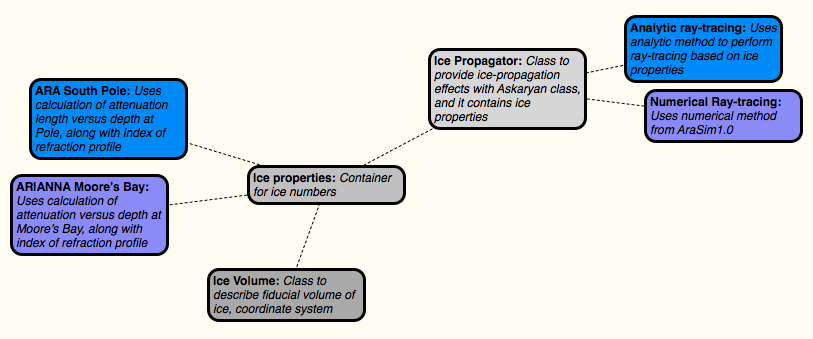
\includegraphics[width=0.9\textwidth]{figures/Propagation.png}
\caption{\label{fig:fig1} The original RF propagation class structure from AraSim2 outline.}
\end{center}
\end{figure}
\end{frame}

\begin{frame}{Class Structure and Functions}
\begin{figure}
\begin{center}
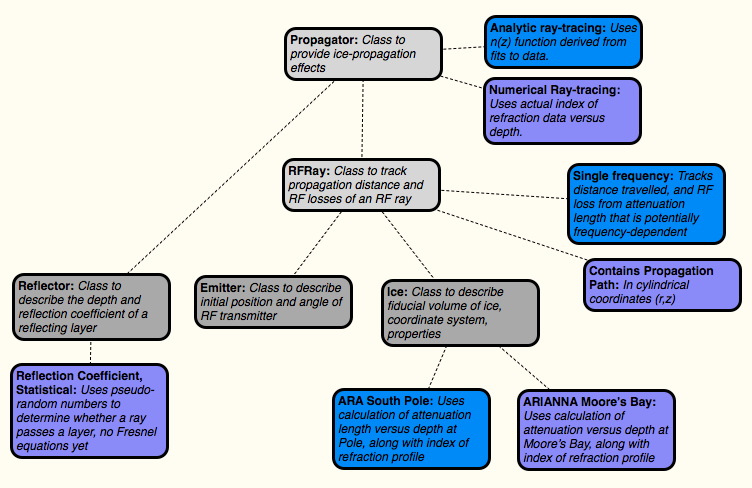
\includegraphics[width=0.8\textwidth]{figures/Propagation2.png}
\caption{\label{fig:fig2} The current RF propagation class structure.}
\end{center}
\end{figure}
\end{frame}

\begin{frame}{How Propagator.h Works}
\begin{verbatim}
std::cout<< i;
\end{verbatim}
\end{frame}

\end{document}